% ============================================================
% §1 问题背景与重述
% 竞赛: 电工杯 B题 (2026) | Stage 08 产物
% ============================================================

\section{问题背景与重述}

\subsection{工程背景}

截至2025年末，我国60岁及以上人口突破3.1亿（22.0\%），失能半失能超4,500万。在"9073"养老格局下，\textbf{嵌入式社区养老服务站}作为"小而精、就近就便"的居家-社区协同模式，正成为破解"养老最后一公里"的主流方案。当前面临三大瓶颈：(1) 老年人口状态退化呈马尔可夫棘轮效应，中长期需求预测高度非线性；(2) 选址-规模-定价三重耦合构成NP-hard联合优化；(3) "公益优先、微利运营"下补贴效率亟待提升。

\subsection{题目重述}

本题以某街道10个连片小区（A--J）为场景，提供5附件数据，要求依次解决四问题：(1) 基于转移概率（自理$\to$半失能4.5\%/半失能$\to$失能10\%/死亡率5\%/新增自理7\%）的Markov人口预测及消费约束需求测算；(2) 预算$\le$120万、半径$\le$1000m下的小/中/大（18/32/45万）服务站选址-规模联合优化；(3) 固化选址下利润率$\le$8\%的6项服务差异化定价；(4) 三场景参数扰动下的鲁棒性检验。

\subsection{数据概览}

该区域常住人口31,300人，60+老人6,864人（老龄化率21.9\%），人均月收入3,250元。距离矩阵对称，20条边$>$1000m。5附件210条记录缺失率0.0\%。

\subsection{技术路线}

整体框架为"预测--选址--定价--灵敏度"四阶段递进（图\ref{fig:tech_route}）：Q1增生型Markov+Leslie双模型互证，输出人口预测CSV供下游模型消费；Q2 MILP-MCLP-ES（McCormick包络+Big-M线性化）固化为选址-规模决策；Q3词典序MILP定价以Q2的$y_{ik}^*$与$x_{ij}^*$为固定输入；Q4三场景6组MILP重求解配合多维度韧性矩阵。

\begin{figure}[H]
\centering
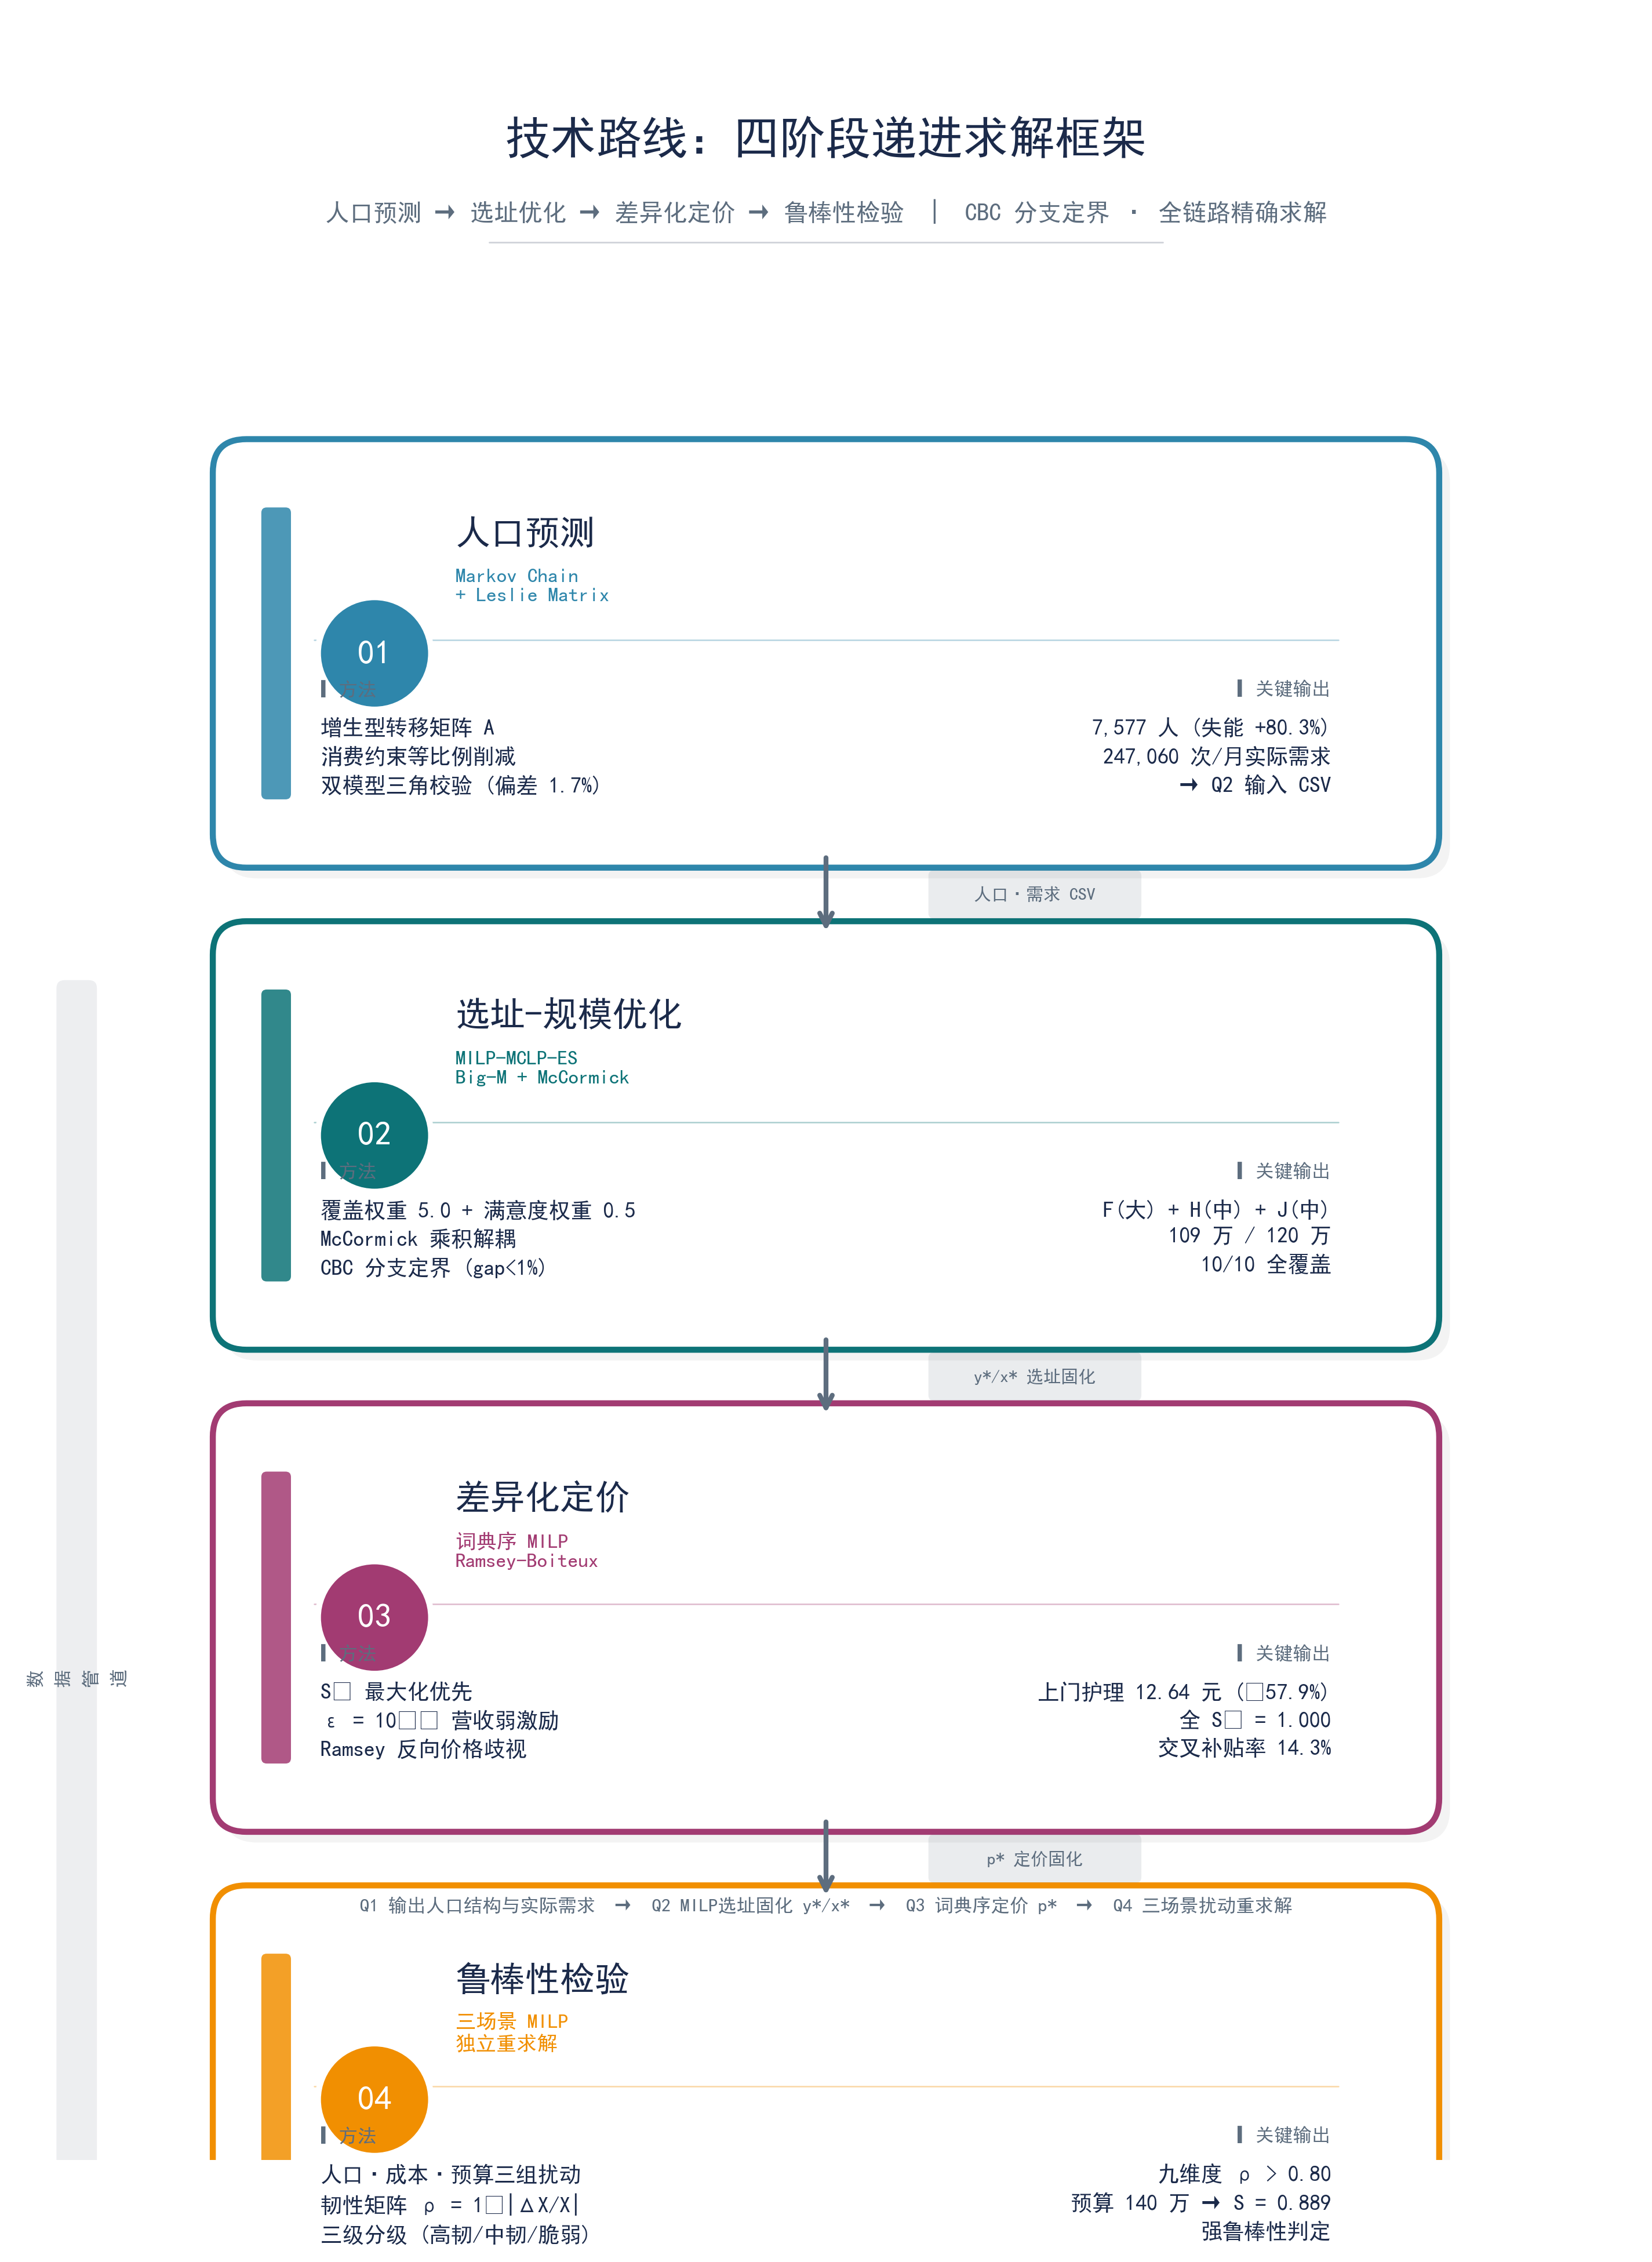
\includegraphics[width=0.92\textwidth]{figures/figure_tech_route.png}
\caption{技术路线：四阶段递进框架——数据流自附件1--5始，经Markov人口预测、MILP选址优化、词典序定价、多场景鲁棒性验证，形成完整的"预测--选址--定价--灵敏度"闭环。}
\label{fig:tech_route}
\end{figure}
